%% Creator: Inkscape inkscape 0.92.2, www.inkscape.org
%% PDF/EPS/PS + LaTeX output extension by Johan Engelen, 2010
%% Accompanies image file 'yke3.eps' (pdf, eps, ps)
%%
%% To include the image in your LaTeX document, write
%%   \input{<filename>.pdf_tex}
%%  instead of
%%   \includegraphics{<filename>.pdf}
%% To scale the image, write
%%   \def\svgwidth{<desired width>}
%%   \input{<filename>.pdf_tex}
%%  instead of
%%   \includegraphics[width=<desired width>]{<filename>.pdf}
%%
%% Images with a different path to the parent latex file can
%% be accessed with the `import' package (which may need to be
%% installed) using
%%   \usepackage{import}
%% in the preamble, and then including the image with
%%   \import{<path to file>}{<filename>.pdf_tex}
%% Alternatively, one can specify
%%   \graphicspath{{<path to file>/}}
%% 
%% For more information, please see info/svg-inkscape on CTAN:
%%   http://tug.ctan.org/tex-archive/info/svg-inkscape
%%
\begingroup%
  \makeatletter%
  \providecommand\color[2][]{%
    \errmessage{(Inkscape) Color is used for the text in Inkscape, but the package 'color.sty' is not loaded}%
    \renewcommand\color[2][]{}%
  }%
  \providecommand\transparent[1]{%
    \errmessage{(Inkscape) Transparency is used (non-zero) for the text in Inkscape, but the package 'transparent.sty' is not loaded}%
    \renewcommand\transparent[1]{}%
  }%
  \providecommand\rotatebox[2]{#2}%
  \ifx\svgwidth\undefined%
    \setlength{\unitlength}{690.59998274bp}%
    \ifx\svgscale\undefined%
      \relax%
    \else%
      \setlength{\unitlength}{\unitlength * \real{\svgscale}}%
    \fi%
  \else%
    \setlength{\unitlength}{\svgwidth}%
  \fi%
  \global\let\svgwidth\undefined%
  \global\let\svgscale\undefined%
  \makeatother%
  \begin{picture}(1,0.83405734)%
    \put(0,0){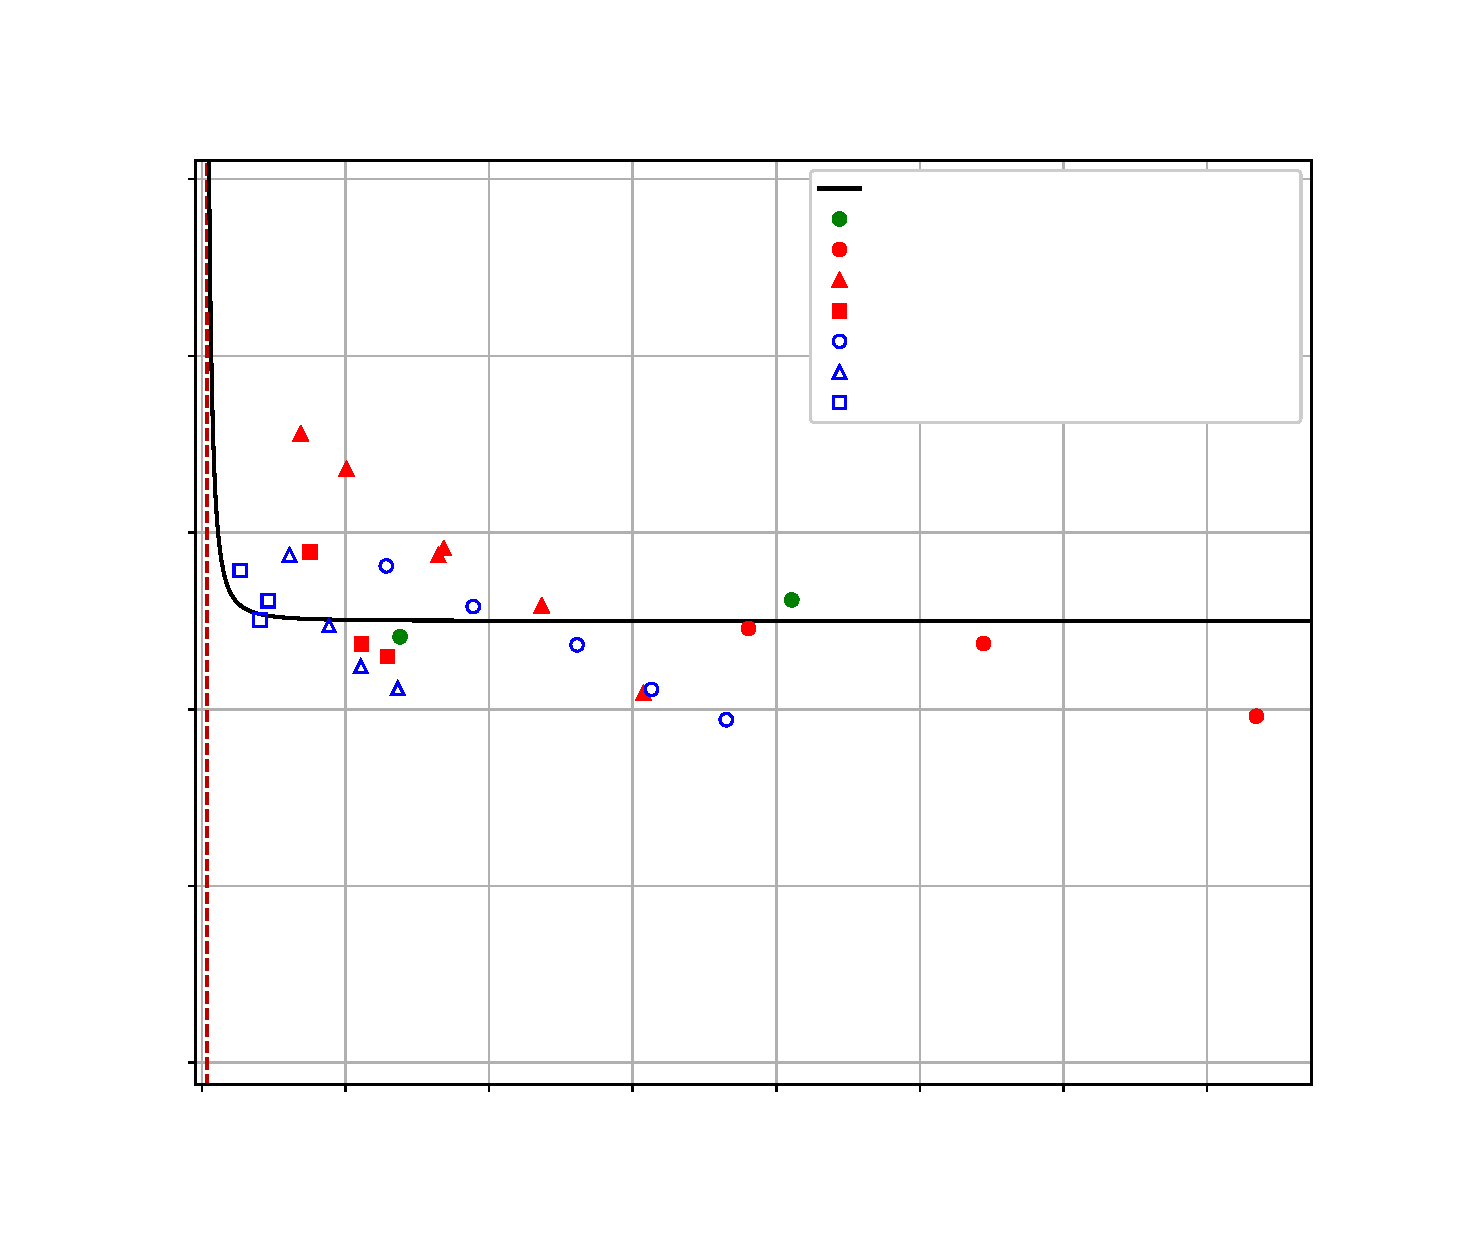
\includegraphics[width=\unitlength]{images_2ddl/yke3.eps}}%
    \put(0.11819679,0.055061454){\color[rgb]{0,0,0}\makebox(0,0)[lb]{\smash{0}}}%
    \put(0.20939183,0.055061454){\color[rgb]{0,0,0}\makebox(0,0)[lb]{\smash{20}}}%
    \put(0.30919056,0.055061454){\color[rgb]{0,0,0}\makebox(0,0)[lb]{\smash{40}}}%
    \put(0.40898928,0.055061454){\color[rgb]{0,0,0}\makebox(0,0)[lb]{\smash{60}}}%
    \put(0.50878801,0.055061454){\color[rgb]{0,0,0}\makebox(0,0)[lb]{\smash{80}}}%
    \put(0.60398349,0.055061454){\color[rgb]{0,0,0}\makebox(0,0)[lb]{\smash{100}}}%
    \put(0.70378222,0.055061454){\color[rgb]{0,0,0}\makebox(0,0)[lb]{\smash{120}}}%
    \put(0.80358094,0.055061454){\color[rgb]{0,0,0}\makebox(0,0)[lb]{\smash{140}}}%
    \put(0.067107124,0.095120895){\color[rgb]{0,0,0}\makebox(0,0)[lb]{\smash{0.0}}}%
    \put(0.067107124,0.2140501){\color[rgb]{0,0,0}\makebox(0,0)[lb]{\smash{0.2}}}%
    \put(0.067107124,0.33689111){\color[rgb]{0,0,0}\makebox(0,0)[lb]{\smash{0.4}}}%
    \put(0.067107124,0.45973212){\color[rgb]{0,0,0}\makebox(0,0)[lb]{\smash{0.6}}}%
    \put(0.067107124,0.58257457){\color[rgb]{0,0,0}\makebox(0,0)[lb]{\smash{0.8}}}%
    \put(0.067107124,0.70541558){\color[rgb]{0,0,0}\makebox(0,0)[lb]{\smash{1.0}}}%
    \put(0.04226991,0.37966696){\color[rgb]{0,0,0}\rotatebox{90}{\makebox(0,0)[lb]{\smash{$E_{p,g}/E_{tot}$}}}}%
    \put(0.59802491,0.70735418){\color[rgb]{0,0,0}\makebox(0,0)[lb]{\smash{\scriptsize modèle théorique 2DDL}}}%
    \put(0.59802491,0.68610889){\color[rgb]{0,0,0}\makebox(0,0)[lb]{\smash{\scriptsize Y\&K acier (120,30)}}}%
    \put(0.59802491,0.6648636){\color[rgb]{0,0,0}\makebox(0,0)[lb]{\smash{\scriptsize Y\&K polyimide (125,10)}}}%
    \put(0.59802491,0.6436183){\color[rgb]{0,0,0}\makebox(0,0)[lb]{\smash{\scriptsize Y\&K polyimide (125,15)}}}%
    \put(0.59802491,0.62237446){\color[rgb]{0,0,0}\makebox(0,0)[lb]{\smash{\scriptsize Y\&K polyimide (125,20)}}}%
    \put(0.59802491,0.60112916){\color[rgb]{0,0,0}\makebox(0,0)[lb]{\smash{\scriptsize Y\&K polyimide (75,10)}}}%
    \put(0.59802491,0.57988387){\color[rgb]{0,0,0}\makebox(0,0)[lb]{\smash{\scriptsize Y\&K polyimide (75,15)}}}%
    \put(0.59802491,0.55863858){\color[rgb]{0,0,0}\makebox(0,0)[lb]{\smash{\scriptsize Y\&K polyimide (75,25)}}}%
    \put(0.47,0.01){\color[rgb]{0,0,0}\makebox(0,0)[lb]{\smash{$F/m_r g$ }}}%
  \end{picture}%
\endgroup%
